\documentclass[a4paper]{article}
\usepackage{graphicx}
\begin{document}
\section{Turing Machines: The Simplest Computers}
\label{sec:simplest} %use the cross referencing feature
Turing machines are the simplest and most widely used theorectical models of computing. Far too slow and unwieldy ever to be embodied in a real device, these conceptual machines nevertheless seem to capture everything we mean by the term \textit{computation}. Not only do Turing machines occupy the top level of the Chomsky hierarchy, but they also seem capable of computing any function which is computable by any other conceptional scheme.

\section{Alan Turing}
The Turing machines described in section \ref{sec:simplest} are named after Alan Turing. %ref =refers to any documents

\section{Accomplishments of Turing}
You can find Turing's publications in Google scholar. \cite{googlescholar} His paper on the Entscheidungsproblem was published in 1937. \cite{alanturing} He wrote about thinking machines in 1950. \cite{turingomnibus}
\begin{figure}
    \centering
    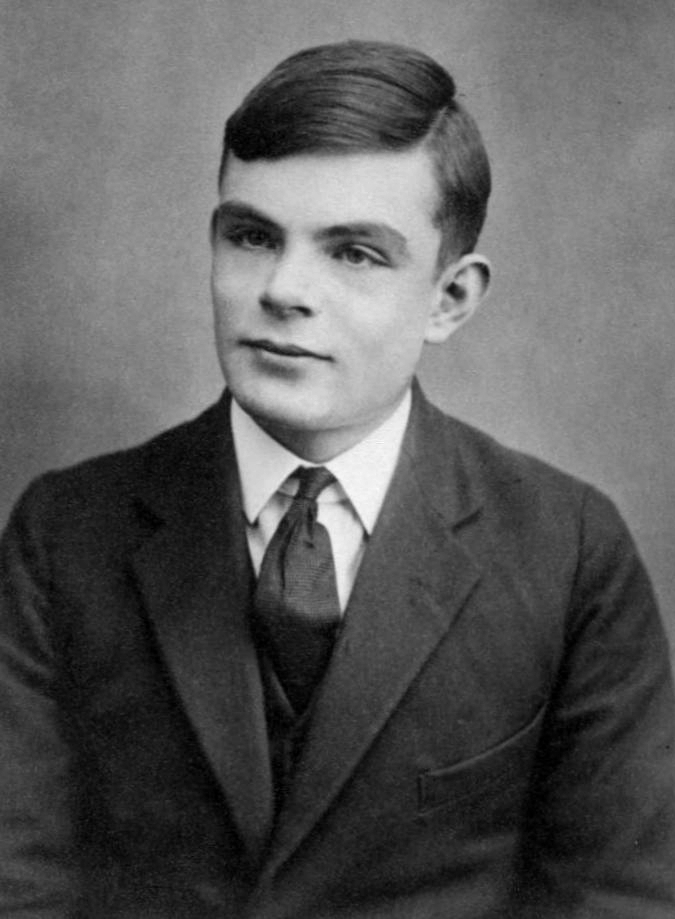
\includegraphics[width=10cm]{turing.jpg}
    \caption{Turing machines are named after Alan Turing}
    \label{figure:turing}
\end{figure}
\bibliographystyle{unsrt}
\bibliography{turing.bib}
\end{document}